\documentclass[11pt]{article} %{{{

\usepackage{amsmath}
\usepackage{amssymb}
\usepackage{graphicx}
\usepackage{url}
\usepackage[usenames,dvipsnames,svgnames,table]{xcolor}
\definecolor{light-gray}{gray}{0.8}
\def \del #1{ {\color{light-gray}{#1}} }
\def\yy#1{\footnote{\color{red}\textbf{#1 -YY}} }
\def\ej#1{\footnote{\color{blue}\textbf{#1 -EJ}} }
\usepackage{hyperref}


\usepackage[backend=bibtex]{biblatex}
\addbibresource{main.bib}
\graphicspath{ {./figs} }

\usepackage{array}
\usepackage{subcaption}
%}}}

\begin{document} %{{{

\title{A Thousand Times over: Novelty and Success of Story Re-creations} %{{{
\date{\today}
\maketitle %}}}

\section{Introduction} %{{{
\label{sec:introduction}

Story telling is one of human beings' basic needs and abilities\cite{gottschall2012storytelling}. Despite having endless forms, most stories can be considered as variations of one of the basic archetypes. In mythology studies, Campbell deduced a fundamental structure, \emph{the hero's journey}, from all major myths around the world \cite{campbell2008hero}. Levi-Strauss broke down different versions of a myth to identify common mythemes \cite{levi1955structural}. In oral legends and tales, many stories had a certain origin and developed into different versions through time and interaction between creators. Myths and folktales in oral traditions of civilizations around the world often follow this pattern, for example, the tale of the \emph{Little Red Riding Hood} originated approximately in the 10th century, and has developed multiple variations\cite{littlered}. Some elements of the legend \emph{Mahabharata} can be traced back to the Vedic period (15--6 century B.C.) as oral tales told by bards, and was textualized into many versions\cite{van2011mahabharata}.


and \emph{Iliad} also followd with this pattern.

In the contemporary pop culture, this tradition is sometimes found in a new form --- fan works. Sometimes defined more formally as transformative works, they are creative works made by fans based on one or more original works, and are often centered around certain characters or story lines\cite{wiki:transf_work}. For example, a story written by a contemporary fan about Sherlock Holmes in his retirement is considered a fan work. Although fan works contain multiple media types such as art, music and games, one of the most common type is creative writing---fanfictions. People interested in such activities often connect and interact with each other, forming communities known as fandoms\cite{wiki:fandom}.

Similar to other creative works, fanfictions are constantly under selection and evaluation of their readers. The most successful fanfictions may be published and even adapted into other media forms (for example, \emph{Fifty Shades of Grey} was originally a fanfiction of \emph{Twilight}). Meanwhile, the majority of them remain mostly unknown.

We study the novelty and success of fanfictions in fandoms using data from Archive of Our Own (AO3). This site hosts fan works --- mainly fanfictions --- that users upload and their metadata, and categorizes them based on fandoms. Established in 2010, it has become one of the most popular transformative work archives. We first show that the novelty of fanfictions has a negative effect on their success -- the more a fiction is different from other fictions, the less it is liked by its readers. Then we show that this negative relation influences how authors create fictions.

%}}}

\section{Results} %{{{
\label{sec:results}
\subsection{Novelty doesn't make fictions popular}
We define novelty as the cosine distance between a fiction and the typical fiction in its fandom. In the correlation matrix shown in figure \ref{fig:corr_heatmap}, we found that the cosine distance has a negative correlation with the hits/kudos that fictions receive. That is, the more creative a fiction is, the less kudos it will receive.

\begin{figure}[htbp]
\begin{center}
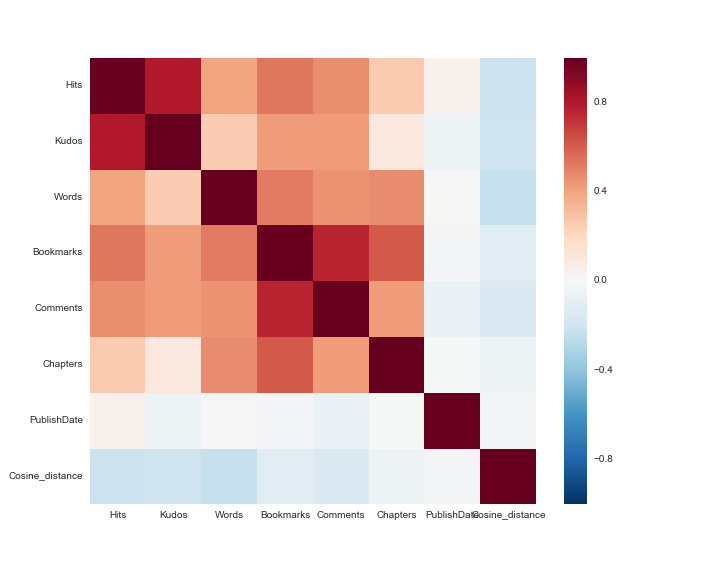
\includegraphics[width=0.8\textwidth]{/corr_heatmap_agg_1000.png}
\caption{Pairwise correlation between some important fields }
\label{fig:corr_heatmap}
\end{center}
\end{figure}

We further investigate this relation by fitting a negative binomial regression model. The result of the regression is summarized in figure \ref{regression_screenshot}. It can be observed that the cosine distance has a significant negative effect on Kudos.

\begin{figure}[htbp]
\begin{center}
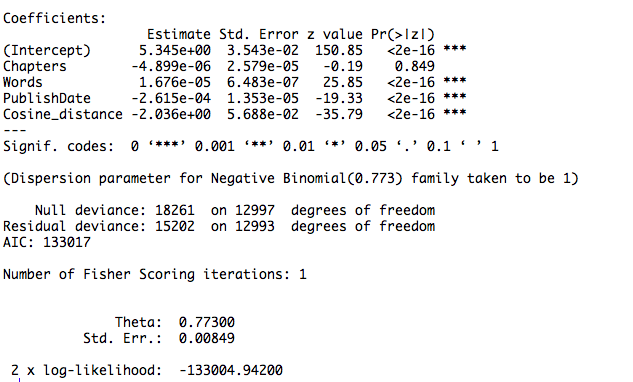
\includegraphics[width=0.8\textwidth]{/regression_screenshot.png}
\caption{Negative binomial regresion results}
\label{fig:regression}
\end{center}
\end{figure}

A closer look into cosine distance and Kudos is shown in figure \ref{fig:cos_kudos}. Because of the long-tailed distribution of Kudos, we choose to look at the log of Kudos. In general, the fandoms show the pattern that the average Kudos decrease when the cosine distance increases.


\begin{figure}[htbp]
\begin{center}
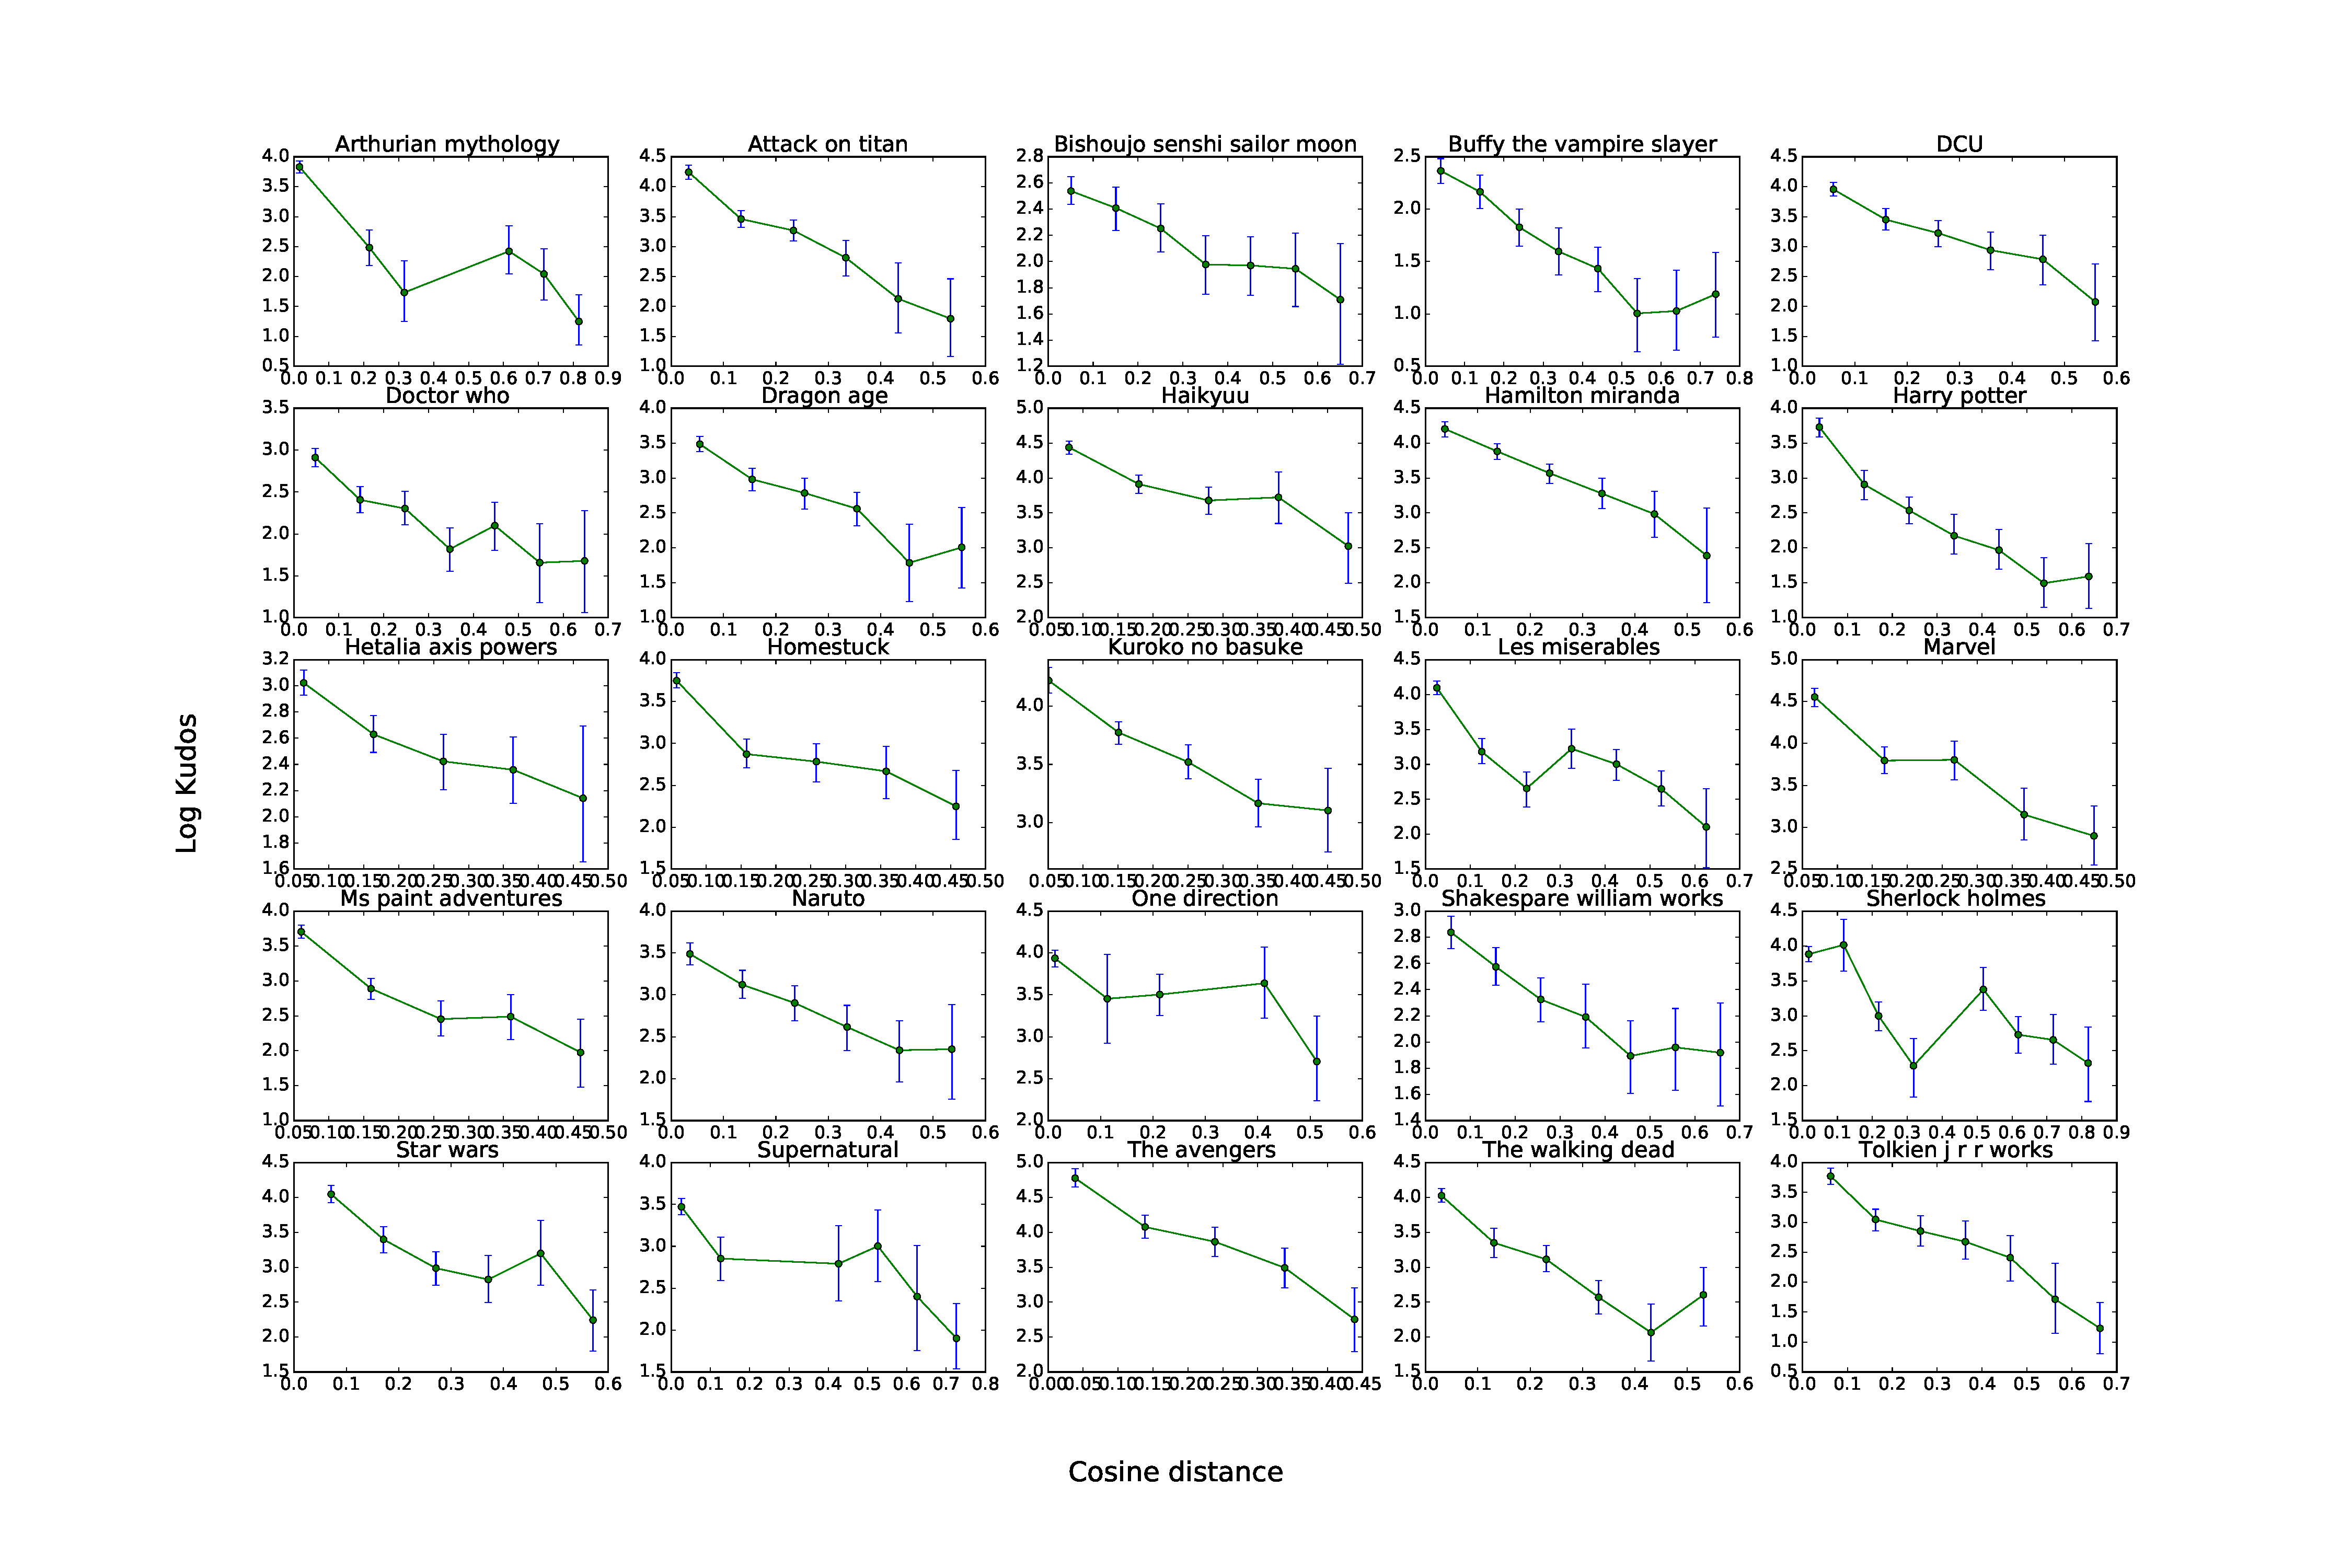
\includegraphics[width=\textwidth]{/cos_log_kudos_agg.pdf}
\caption{Cosine distance and the log of kudos.}
\label{fig:cos_kudos}
\end{center}
\end{figure}


%\subsection{The fandoms grow less creative?}


%}}}



\section{Methods} %{{{
\label{sec:methods}

%}}}

\subsection{Data}
We collected fanfictions from 50 fandoms according to AO3's list of most popular fandoms as of March 2016 \footnote{from this list: \url{http://archiveofourown.org/media}}. To avoid duplication, we remove fandoms with heavy overlapping (e.g.: we keep \emph{Marvel} and removed \emph{Marvel movies}). Fandoms that cover diverse topics (e.g.\emph{k-pop}) are also removed. Finally, we only kept the fictions written in English. This leaves us with 904,760 fictions from 25 fandoms. The number of fictions in each fandom is shown in Figure \ref{fig:fandom_size}.

\begin{figure}[htbp]
\begin{center}
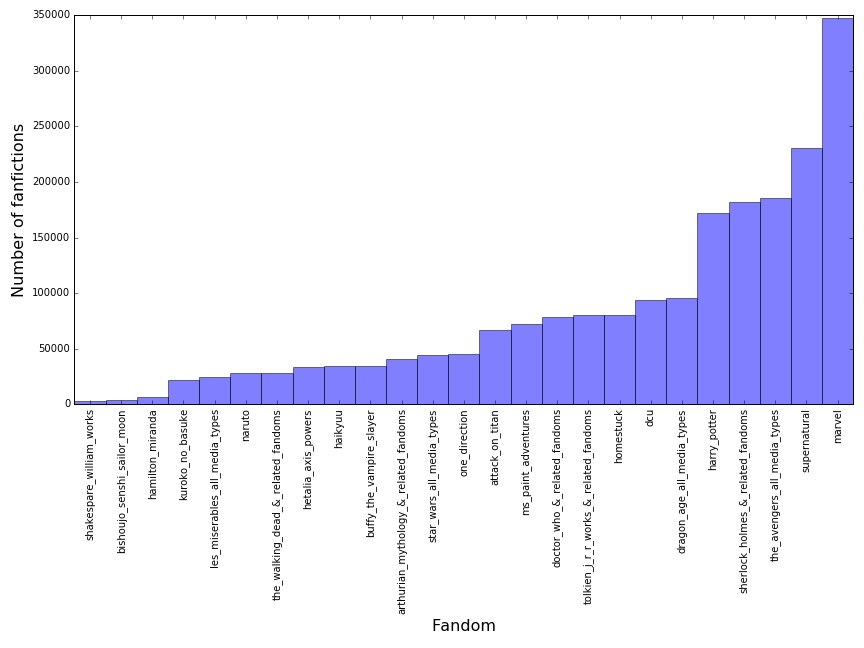
\includegraphics[width=0.9\textwidth]{/fandom_size.png}
\caption{Number of fanfictions in each fandom}
\label{fig:fandom_size}
\end{center}
\end{figure}


Besides the work texts, we also collected metadata including 23 fields. We only used information contained in some of these fields. Table \ref{tab:metadata} gives the names and descriptions of these fields. 

\begin{table}[htp]
\caption{Metadata of the writings}
\begin{center}
\begin{tabular}[width=0.8\textwidth]{p{2cm}|p{4cm}|p{5cm}}
  \hline			
 Fields & Description & Usage\\ 
   \hline			
Text & The fiction texts. & All text analysis are carried out on these texts.\\\hline
Title & Titles of the fictions. & Used to identify the fictions. \\\hline
Fandoms & Describes which fandom(s) the fiction belongs to. & Used to categorize the fictions.\\\hline
Author & The author of the fiction. & Used for identifying the fictions and for text analysis. \\\hline
% Hits & The number of times a fiction is clicked on. & A metric for evaluating the fiction's popularity. \\\hline
Kudos & The number of times that readers "like" the fiction. &  A metric for evaluating the fiction's popularity.\\\hline
Publish Date & The date the fiction was published. & We use this to determine what time period a fiction belongs to. We also use the time between publish and now to evaluate the ``age" of a fiction.\\\hline
Chapters & The number of chapters that a fiction has. \\\hline
Words & The number of words in a fiction.\\\hline

\hline
\end{tabular}
\end{center}
\label{tab:metadata}
\end{table}%

Among the metadata fields, we're especially interested in the fields ``Hits" and ``Kudos", which shows how many times a fiction has been clicked or liked by readers. These are useful proxies for the popularity of a piece of work in a specific fandom.
Both statistics have power-law-like distribution, as shown in  Figure \ref{fig:long_tail}, proving our conception that the popularity of fictions is very imbalanced: most fictions are rarely read and receive little Kudos, while very few get the majority of views and Kudos.

\begin{figure}[htbp]
\begin{center}
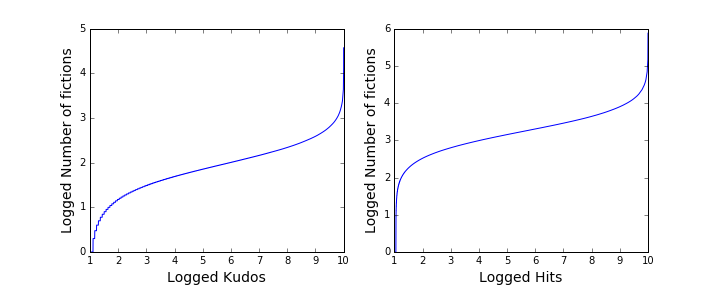
\includegraphics[width=\textwidth]{/kudos_hits_dist.png}
\caption{Log-log CCDF of the distribution of Kudos and Hits.}
\label{fig:long_tail}
\end{center}
\end{figure}

\subsection{Language model}
We model the fictions with a unigram language model. The Simple Good-Turing smoothing\cite{gales1995good} is applied to improve the model, and to assign non-zero probabilities to previously unseen unigrams. When creating the set of unigrams, we also remove the rare unigrams that appear in less than 5 documents and left out fictions with less than 500 words.

We verify that this model successfully captures the semantic and stylometrical contents of fictions. Using this model, the fictions from the same author are more close to each other compared to fictions from different authors, measuring by cosine distance, as shown in Figure \ref{fig:comparison_unigram_sgt}.

\begin{figure}[htbp]
\begin{center}
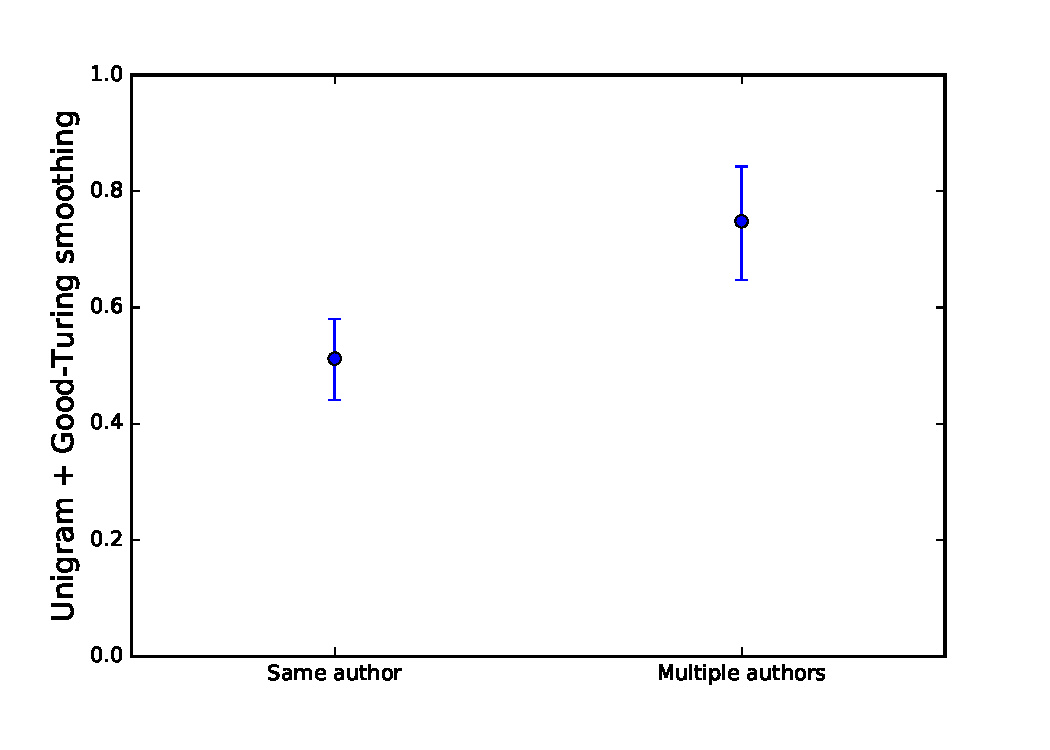
\includegraphics[width=0.6\textwidth]{/comparison_unigram_sgt.pdf}
\caption{Cosine distances between fictions from the same author and fictions from different authors in the Shakespeare fandom.
Left: The average cosine distance between fictions from same authors. In a 10-author dataset, average pairwise cosine distances between fictions from each author is calculated, and the overall distance is the average of the 10 groups. Right: The computation repeated on 10 random groups with the same size. The error bars are computed with the bootstrap resampling method. }
\label{fig:comparison_unigram_sgt}
\end{center}
\end{figure}

We further define the concept of a \emph{typical} fiction. A typical fiction of a fandom is the average of probability distributions of all fictions in the fandom. This allows us to calculate the distance between any fiction and the typical fiction. 

\subsection{Regression}
We apply a negative binomial regression using R's MASS library. 










\printbibliography
    
\end{document} %}}}
